\chapter{Design} %\label{1cap:spinta_laterale}
% [titolo ridotto se non ci dovesse stare] {titolo completo}
%
\begin{citazione}
\end{citazione}



\section{Obiettivi}
Questo capitolo mostra le scelte di design e lo sviluppo di Yumi. Lo scopo è quello di creare un bot a supporto degli sviluppatori che permetta di suggerire al programmatore una possibile funzione implementabile attraverso l'utilizzo di un'interfaccia che accetti un input e restituisca la funzione in output.
Grandi modelli basati su linguaggio naturale hanno dimostrato grandi progressi nella neural program synthesis e task correlati. Le scelte di creazione del nostro program synthesis andavano in due direzioni diverse. L'utilizzo di modelli pre-addestrati e delle loro Api con l'aggiunta del nostro dataset accorpato a quello già presente, oppure un approccio diverso basato sulla similiarità del testo in input con quello ricercato.
Tuttavia la prima soluzione avrebbe portato a diverse difficoltà:
\begin{itemize}
    \item l'impossibilità di utilizzo di alcuni framework che avrebbero reso possibile questa scelta
    \item l'impossibilità di utilizzo del nostro calcolatore per il training in quanto la potenza di calcolo necessaria non era sufficente
    \item l'impossibilità di trovare la mole di dati necessaria ad utilizzare il fine-tuning 
\end{itemize}
Pertanto, si è deciso di affrontare il problema in esame mediante tecniche di Machine Learning che permettessero di effettuare un calcolo basato sulla similarità dei vari elementi.
\section{Funzionalità e processo di sviluppo}
In questo paragrafo si esaminerà il modello di sviluppo e i casi d'uso di Yumi, nello specifico i due casi d'uso GetConcreteConversation e GetRandomConversation e il modello di sviluppo Test-Driven Development utilizzato per la scrittura del codice. Il sistema proposto è un software scritto in Flutter che ha lo scopo di aiutare lo sviluppatore nella ricerca di una determinata funzione basandosi su un testo da lui scritto.



\subsection{Casi d'uso}
In questo paragrafo verranno mostrati i casi d'uso per Yumi. I casi d’uso (use cases) sono descrizioni di come può essere usato un sistema, servono a raccogliere i requisiti del software in maniera esaustiva e non ambigua, focalizzandosi sugli attori che interagiscono col sistema, valutandone le varie interazioni. 

L'attore principale in questo caso è proprio l'utente. Esso avrà la possibilità di effettuare delle query al modello del nostro conversational agent e ricevere da lui delle risposte. Un'altra funzionalità è quella di ricevere delle risposte randomiche, quest'ultima pensata perlopiù per valutarne le potenzialità e l'effettiva funzionalità.

Il secondo attore per l'appunto è il sistema, le cui funzionalità, derivate dai requisiti funzionali, vengono descritte tramite i casi d'uso.

In Yumi abbiamo due casi d'uso:
\begin{itemize}
    \item \textbf{GetConcreteConversation}:  Che servirà per ottenere, dato un input, in output da parte del modello il relativo blocco di codice più consono a quanto richiesto dall'utente. Questo è il caso d'uso principale del nostro conversational agent, in quanto sfrutta tutte le funzionalità per il quale è stato creato, ovvero la predizione del blocco di codice dall'input dell'utente. (Tabella \ref{tab:tabella-getconcreteconversation})
    \item \textbf{GetRandomConversation}: Che servirà per ottenere, in output da parte del modello un blocco di codice ricavato in modo randomico da parte del modello all'interno del nostro dataset. Questo caso d'uso è stato creato per scopi scientifici, sarà utilizzato principalmente per testare il corretto funzionamento del conversational agent e delle API ad esso legate e valutarne le potenzialità.(Tabella \ref{tab:tabella-getrandomconversation})
\end{itemize}
\begin{table}[hp]
    \renewcommand\arraystretch{1.5}
    \newcommand\mcl[1]{\multicolumn{4}{l}{#1}}
    \centering
    \caption{Tabella Caso d'uso GetConcreteConversation}
    \label{tab:tabella-getconcreteconversation}
    \begin{tabularx}{\textwidth}{llXXl}
        \toprule
        \textbf{Use Case \#1}       & \mcl{\textbf{GetConcreteConversation}}                                                                                            \\ \toprule
        Descrizione                 & \mcl{Ottenere il codice di una funzione}                                                                                          \\ \midrule
        Entry Condition             & \mcl{L'utente deve trovarsi nella schermata principale}                                                                           \\ \midrule
        Exit on Success             & \mcl{La piattaforma restituisce in output un blocco di codice}                                                                    \\ \midrule
        Exit on Failure             & \mcl{La piattaforma restituisce un messaggio di errore}                                                                           \\ \midrule
        Attore Primario             & \mcl{Utente}                                                                                                                      \\ \midrule
        Trigger                     & \mcl{Inserimento dell'input e pressione del comando}                                                                              \\ \midrule
        \textsc{Flusso di Eventi}   & \textbf{Step} & \textbf{Attore 1}                                 & \textbf{Sistema}                                              \\ \cline{2-5}
                                    & 1             & L'utente usa il comando per scrivere un commento  &                                                               \\ \cline{2-5}
                                    & 2             &                                                   & Il sistema     \\ \midrule
        \textsc{Flusso Alternativo} & \textbf{Step} & \textbf{Attore 1}                                 & \textbf{Sistema}                                              \\ \cline{2-5}
                                & 1             & L'utente usa il comando per scrivere un commento  &                                                                   \\ \cline{2-5}
                                    & 2             &                                                   & Il sistema mostra un messaggio di errore                      \\ \midrule
        \textsc{Note}         & \mcl{} \\
                               &         &                    &               &  \\
        \bottomrule
    \end{tabularx}
\end{table}

\begin{table}[hp]
    \renewcommand\arraystretch{1.5}
    \newcommand\mcl[1]{\multicolumn{4}{l}{#1}}
    \centering
    \caption{Tabella Caso d'uso GetRandomConversation}
    \label{tab:tabella-getrandomconversation}
    \begin{tabularx}{\textwidth}{llXXl}
        \toprule
        \textbf{Use Case \#1}  & \mcl{\textbf{GetRandomConversation}}                                   \\ \toprule
        Descrizione        & \mcl{Ottenere il codice casuale di una funzione}                                \\ \midrule
        Entry Condition          & \mcl{L'utente deve trovarsi nella schermata principale}               \\ \midrule
        Exit on Success & \mcl{La piattaforma restituisce in output un blocco di codice casuale}        \\ \midrule
        Exit on Failure  & \mcl{La piattaforma restituisce un messaggio di errore}                       \\ \midrule
        Attore Primario          & \mcl{Utente}                       \\ \midrule
        Trigger                & \mcl{Pressione del comando per l'output casuale}   \\ \midrule
        \textsc{Flusso di Eventi}   & \textbf{Step} & \textbf{Attore 1}        & \textbf{Sistema} \\ \cline{2-5}
                               & 1             & L'utente usa il comando per ottenere un commento casuale       & \\ \cline{2-5}
                               & 2             &                          & Il sistema mostra il blocco di codice relativo al commento \\ \midrule
        \textsc{Flusso Alternativo} & \textbf{Step} & \textbf{Attore 1}        & \textbf{Sistema} \\ \cline{2-5}
                               & 1             & L'utente usa il comando per ottenere un commento casuale       & \\ \cline{2-5}
                               & 2             &                          & Il sistema mostra mostra un messaggio di errore \\ \midrule
        \textsc{Note}         & \mcl{} \\
                               &         &                    &               &  \\
        \bottomrule
    \end{tabularx}
\end{table}



\subsection{Modello di Sviluppo}
Si è scelto di seguire un modello di sviluppo Test-Driven Development (abbreviato TDD) che prevede che la creazione di test avvenga prima della scrittura del software che deve essere sottoposto a test. Più in dettaglio il TDD prevede la ripetizione di un breve ciclo di sviluppo in tre fasi, detto "Ciclo TDD" (Figura \ref{fig:tdd}). 
\begin{figure}[h]
    \centering
    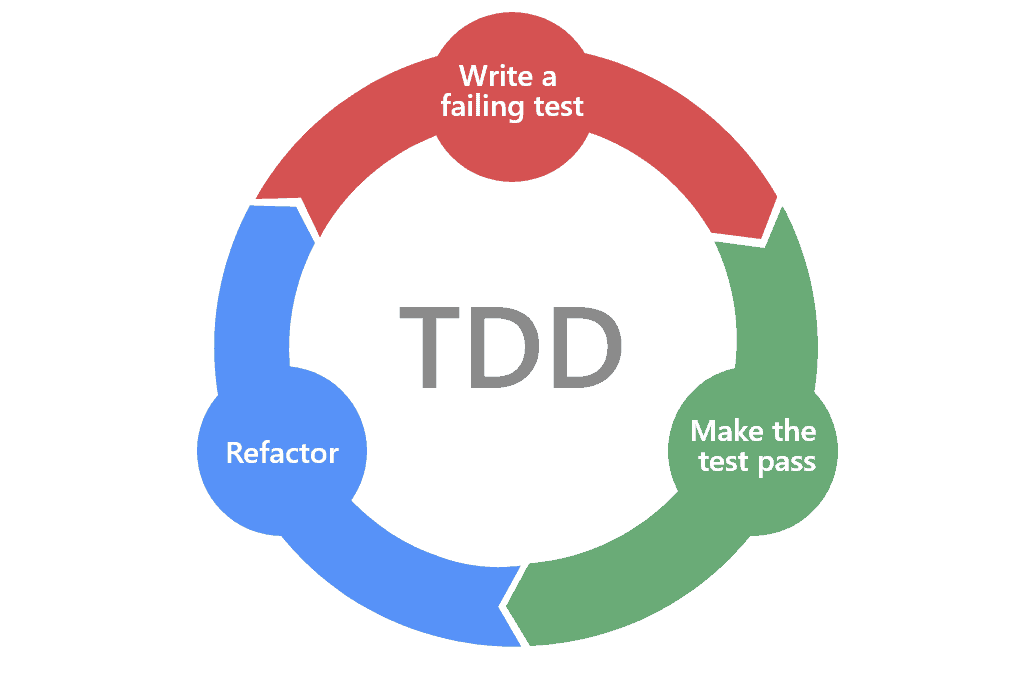
\includegraphics[scale=.35]{immagini/tdd.png}
    \caption{Le tre fasi del Test-Driven Development}
    \label{fig:tdd}
\end{figure}
\begin{itemize}
    \item \textbf{Red Phase}: In questa fase viene scritto un test, nel nostro caso in flutter utilizzando il package \texttt{flutter\_test/flutter\_test.dart}, volto a validare la funzionalità da implementare. Una volta completato il test che descrive la funzionalità che verra implementata, deve essere eseguito e all'esecuzione dovrà produrre un errore (si dice che il test è Rosso/Red). In questo momento la fase è completata e si passa alla successiva del ciclo.
    \item \textbf{Green Phase}: In questa fase si implementa la funzionalità con la minima quantità di codice possibile volto a far si che il test passi (si dice che il test è Verde/Green). Il codice non deve essere di qualità, e deve focalizzarsi sullo sviluppo della parte necessaria a far passare il test, infatti è vietato nello sviluppo TDD aggiungere codice che non è finalizzato al superamento del test. In questa fase inoltre si eseguono anche tutti i test precedenti per far si che la funzionalità appena creata non abbia intaccato parti di funzionalità precedentemente scritte. Quando tutto è Verde (Green) si passa alla fase successiva.
    \item \textbf{Refactoring Phase}: Quando tutti i test sono Verdi si passa al refactoring del codice, ovvero a migliorare la sua leggibilità e struttura attraverso un procedimento basato su piccole modifiche, per esempio, l'eliminazione del codice duplicato, la semplificazione di cicli, rinominare variabili e funzioni etc. L'obiettivo non è quello di ottenere codice perfetto ma solo di migliorarne la struttura.
\end{itemize}

\begin{lstlisting}[language=dart,caption=Un esempio di test all'interno del progetto per la creazione del modello]
import 'dart:convert';

import 'package:flutter_test/flutter_test.dart';
import 'package:yumi/features/conversation/data/models/conversation_model.dart';
import 'package:yumi/features/conversation/domain/entities/conversation.dart';

import '../../../../fixtures/fixture_reader.dart';
void main() {
    const tConversationModel = ConversationModel(number: 1, text: 'Test Text');
    group('fromJson', () {
        test(
          'should return a valid model wheen the JSON number is an integer',
          () async {
            // arrange
            final Map<String, dynamic> jsonMap =
                json.decode(fixture('conversation.json'));
            // act
            final result = ConversationModel.fromJson(jsonMap);
            // assert
            expect(result, tConversationModel);
          },
        );
      });
    }
}
\end{lstlisting}

L'applicazione del TDD porta in generale allo sviluppo di un numero maggiore di test e a una maggiore ed è stato possibile applicarlo al progetto in quanto è abbastanza semplice da fare in questo caso, trattandosi di un software minimale. Infatti, se da un lato il TDD permette di scrivere un'applicazione quasi esente di bug, dall'altro il tempo impiegato per portare a termine la creazione di una funzionalità aumenta, soprattutto in team piccoli.





\section{Il Dataset}
Il dataset necessario al modello di intelligenza artificiale per suggerire un possibile output in base al commento in input è stato generato selezionando i repository GitHub da un'ampia raccolta di repository. Queste repository sono state raccolte da SEART-GithubSearch \url{https://seart-ghs.si.usi.ch/}\cite{Dabic:msr2021data}. L'obiettivo di questo dataset è fornire un set di addestramento per il preaddestramento di modelli linguistici di grandi dimensioni su dati di codice per aiutare i ricercatori di ingegneria del software a comprendere meglio il loro impatto sulle attività relative al software, come il completamento automatico del codice. Contiene principalmente codice Dart, ma sono inclusi anche altri linguaggi di programmazione in varia misura.
È stato il lavoro più importante ed anche il più delicato in quanto ha richiesto numerose ore tra la ricerca dei tool adatti all'esportazione dei dati, l'esportazione dei dati stessi che come vedremmo superano gli 80Gb, fino alla creazione degli script di ingegnerizzazione degli stessi.
\subsection{Struttura del Dataset}
In questa sezione andiamo ad esaminare la struttura del dataset risultante.
\begin{lstlisting}[language=json,firstnumber=1]
{
  "id": datasets.Value("int64"),
  "comment": datasets.Value("string"),
  "commentSize": datasets.Value("int64"),
  "code": datasets.Value("string"),
  "codeSize": datasets.Value("int64"),
  "repo": datasets.Value("string"),
}
\end{lstlisting}
I campi del dataset mostrati nel formato json di cui sopra sono identificati in:
\begin{itemize}
    \item \textbf{id}: Identificatore unico per il dato.
    \item \textbf{comment}: Il testo del commento associato alla funzione.
    \item \textbf{commentSize}: La lunghezza in caratteri, spazi inclusi, del commento.
    \item \textbf{code}: Il testo della funzione descritta dal commento.
    \item \textbf{codeSize}: La lunghezza in caratteri, spazi inclusi, del codice.
    \item \textbf{repo}: Il nome della repository GitHub dalla quale è stato estratto.
\end{itemize}

\subsection{Creazione del Dataset}
Il primo passo è stato quello di estrapolare da SEART-GithubSearch il CSV contenente i dati delle repository che combaciavano con la ricerca effettuata utilizzando i seguenti criteri:
\begin{itemize}
    \item >10 GitHub stars
    \item >5 commits
    \item Must have license
    \item Exclude Forks
    \item Language: Dart
\end{itemize}

\begin{figure}[htbp]
\centerline{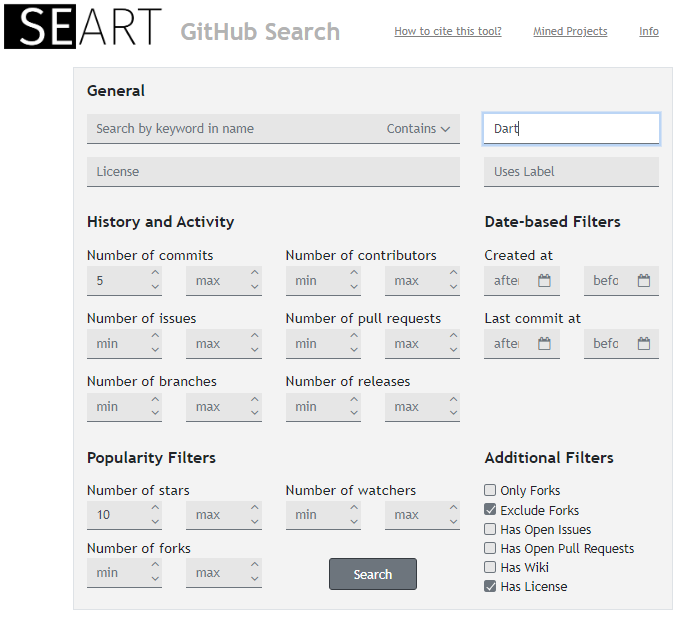
\includegraphics[scale=.85]{immagini/SEARTGithubSearch.png}}
\caption{Interfaccia Web di SEART-GithubSearch \url{https://seart-ghs.si.usi.ch/}\cite{Dabic:msr2021data}.}
\label{fig}
\end{figure}

Il file estrapolato è suddiviso in questo modo:
\texttt{name, isFork, commits, branches, defaultBranch, releases, contributors, license ...}
da questo è stato creato un secondo file CSV \texttt{github\_dart\_repo.csv} necessario all'estrazione che conterrà solamente l'attributo \texttt{name} relativo a \texttt{autore\textbackslash nomeProgetto} della repository GitHub.

Successivamente si è passati alla clonazione di tutte le repository utilizzando uno script in Python di cui riportiamo una parte del codice:

\begin{python}
absolute_path = os.path.dirname(os.path.abspath(__file__))
def download_repo(repo):
    file_name = repo.split("/")[-1]
    if file_name not in os.listdir("output/"):
        os.system(f'git clone --depth 1 --single-branch https://github.com/{repo} output/{file_name}')
    else:
        print(f"Already downloaded {repo}")
with open('github_dart_repo.csv', 'r') as f:
    csv_reader = csv.reader(f)
    repositories = list(map(tuple, csv_reader))
if 'output' not in os.listdir():
    os.makedirs('output')
repo_names = [repo[0] for repo in repositories]
Parallel(n_jobs=40, prefer="threads")(
    delayed(download_repo)(name) for name in tqdm(repo_names))
\end{python}
\begin{lstlisting}[frame=none,caption={Codice python per il clone automatico delle repository\protect\footnote{Codice python per il clone automatico delle repository}},captionpos=b,label=pythonclonegithub]
\end{lstlisting}

Questo script ha generato in una cartella di output tutti i file presenti nelle repository dai quali sono stati poi filtrati i file dart e dai quali sono stati esportati tutti i commenti.
\begin{python}
ext = ('.dart')
def extractdata():
    i=0
    for root, dirs, files in tqdm(os.walk(directory)):
        for filename in files:
            if filename.endswith(ext):
                path = os.path.join(root, filename)
                parseFileComments(path)
                if len(arrayOfText) > 0:
                    saveComments(repo)
\end{python}
\begin{lstlisting}[frame=none,caption={Un'estratto del codice per l'estrazione dei commenti dai file \texttt{.dart}},captionpos=b,label=pythonextractcomment]
\end{lstlisting}
Per dare un'idea del massivo lavoro presente nella costruzione del dataset, nella Figura \ref{figexplorer} è mostrato il totale dei dati grezzi su cui è stato effettuato il lavoro per estrarre i commenti e il codice relativo:
\begin{figure}[h!]
\centerline{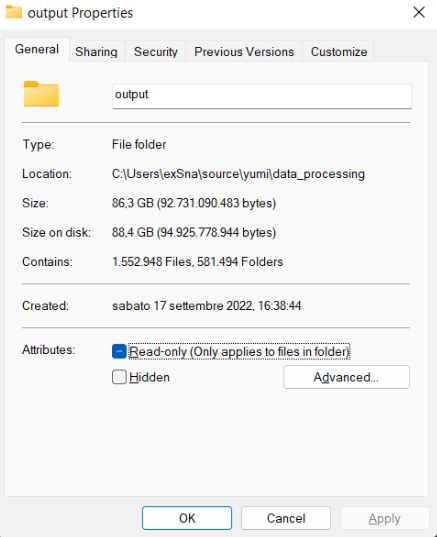
\includegraphics[scale=.75]{immagini/outputFolderProperties.png}}
\caption{Proprietà della cartella Output generato da explorer di Windows}
\label{figexplorer}
\end{figure}
\subsection{Ingegnerizzazione dei dati}
Nella prima fase di ingegnerizzazione dei dati, essi sono stati analizzati per valutarne la validità andando ad eliminare file non relativi a codice.
Sono stati elaborati mediante uno script in Python presente nella repository sotto "datacleaning.py" che è stato utilizzato per l'estrazione dei campi elencati precedentemente, da ogni singolo file con estensione .dart, lo script ha poi generato un file di tipo .csv in cui ogni riga del file è associata ad una riga del dataset.
Nella seconda fase sono stati analizzati ed eliminati file duplicati mediante uno script in python presente nella repository "deduplication.py", lo script puo essere utilizzato da riga di comando:
\begin{center}
\texttt{deduplication.py --data\_dir <data\_dir> --output\_dir <output\_dir>}
\end{center}
Il tool assume che due file sono duplicati se hanno la stessa sequenza di variabili.

I file in input presenti nella directory devono essere in formato \texttt{jsonl}. Il tool caricherà ogni file, trasformerà il codice ottenuto in token, ovvero una lista di variabili all'interno del codice. 

Le variabili sono ottenute mediante regex di token che non sono di tipo alfanumerico, esse vengono poi utilizzate per scovare duplicati negli altri file. In output ci saranno solo i file che non contengono le stesse variabili.

Un ulteriore cleaning del dataset é stato effettuato eliminando codice pre-generato dagli IDE, come per esempio il codice di generazione di un nuovo progetto. Ottenendo quello che è poi il dataset finale sul quale andremo a lavorare. Nella tabella \ref{tab:dataset-table} è presente un esempio, generato dal comando \texttt{df.sample(n = 10).sort\_index()},  delle righe del dataset.

Va fatta una precisazione, i dati sono stati collezionati da repository pubbliche, esiste il rischio che siano presenti informazioni sensibili che gli sviluppatori hanno lasciato all'interno del codice in modo involontario quali secrets key, password, API keys, email, etc. Questo non e' stato oggetto di controllo in quanto, dopo una breve ricerca, non é stato trovato alcun modulo in grado di effettuare un controllo di questo tipo in breve tempo sulla mole di dati a disposizione.

\begin{table}[h]
\tiny
\begin{tabular}{
>{\columncolor[HTML]{383838}}r 
>{\columncolor[HTML]{383838}}r 
>{\columncolor[HTML]{383838}}r 
>{\columncolor[HTML]{383838}}r 
>{\columncolor[HTML]{383838}}r }
{\color[HTML]{D5D5D5} \textbf{comment}} &
  {\color[HTML]{D5D5D5} \textbf{size}} &
  {\color[HTML]{D5D5D5} \textbf{code}} &
  {\color[HTML]{D5D5D5} \textbf{size}} &
  {\color[HTML]{D5D5D5} \textbf{repo}} \\
  {\color[HTML]{D5D5D5} Video mirror mode.\textbackslash{}n\textbackslash{}n} &
  {\color[HTML]{D5D5D5} 29} &
  {\color[HTML]{D5D5D5} @JsonEnum(alwaysCreate: true)\textbackslash{}n} &
  {\color[HTML]{D5D5D5} 31} &
  {\color[HTML]{D5D5D5} agoraio/agora-flutter-sdk} \\
  {\color[HTML]{D5D5D5} Persists in-memory changes to a file on di...} &
  {\color[HTML]{D5D5D5} 51} &
  {\color[HTML]{D5D5D5} class JsonFileService extends Service\textless{}String, ...} &
  {\color[HTML]{D5D5D5} 437} &
  {\color[HTML]{D5D5D5} angel-dart/angel} \\
  {\color[HTML]{D5D5D5} Minimum contrast ratio} &
  {\color[HTML]{D5D5D5} 150} &
  {\color[HTML]{D5D5D5} const minimumTextContrast = 4.5;\textbackslash{}n} &
  {\color[HTML]{D5D5D5} 34} &
  {\color[HTML]{D5D5D5} angulardart/angular\_components} \\
  {\color[HTML]{D5D5D5} Minimum values breakpoints for {[}DeviceScre...} &
  {\color[HTML]{D5D5D5} 147} &
  {\color[HTML]{D5D5D5} const defaultMinimumBreakPoints = ScreenBreakp...} &
  {\color[HTML]{D5D5D5} 69} &
  {\color[HTML]{D5D5D5} jamescardona11/argo} \\
  {\color[HTML]{D5D5D5} Class to expose a stream of {[}Set\textless{}AtKey\textgreater{}{]} b...} &
  {\color[HTML]{D5D5D5} 986} &
  {\color[HTML]{D5D5D5} class SetKeyStream\textless{}T\textgreater extends KeyStreamIterabl...} &
  {\color[HTML]{D5D5D5} 64} &
  {\color[HTML]{D5D5D5} atsign-foundation/at\_client\_sdk} \\
  {\color[HTML]{D5D5D5} Parses english relative time that's in for...} &
  {\color[HTML]{D5D5D5} 538} &
  {\color[HTML]{D5D5D5} DateTime parseEnglishRelativeTime(\textbackslash{}n} &
  {\color[HTML]{D5D5D5} 36} &
  {\color[HTML]{D5D5D5} edwardez/bangumin} \\
  {\color[HTML]{D5D5D5} Fibonacci function ...} &
  {\color[HTML]{D5D5D5} 127} &
  {\color[HTML]{D5D5D5} int fibonacci(int n) => n <= 2 ? 1 :...} &
  {\color[HTML]{D5D5D5} 388} &
  {\color[HTML]{D5D5D5} letsar/binder} \\
  {\color[HTML]{D5D5D5} A person's or business card...} &
  {\color[HTML]{D5D5D5} 70} &
  {\color[HTML]{D5D5D5} class ContactInfo \{\textbackslash{}n Gets contact person...} &
  {\color[HTML]{D5D5D5} 1422} &
  {\color[HTML]{D5D5D5} yanshouwang/camerax} \\
  {\color[HTML]{D5D5D5} class for InterSegmentPointer} &
  {\color[HTML]{D5D5D5} 64} &
  {\color[HTML]{D5D5D5} class InterSegmentPointer extends Pointer \{\textbackslash{}n ...} &
  {\color[HTML]{D5D5D5} 600} &
  {\color[HTML]{D5D5D5} jonaswanke/capnproto-dart} \\
  {\color[HTML]{D5D5D5} SQL\_AUTOCOMMIT options\textbackslash{}n} &
  {\color[HTML]{D5D5D5} 27} &
  {\color[HTML]{D5D5D5} const int SQL\_AUTOCOMMIT\_OFF = 0;\textbackslash{}n} &
  {\color[HTML]{D5D5D5} 39} &
  {\color[HTML]{D5D5D5} jcmellado/dart-odbc}
\end{tabular}
\caption{\label{tab:dataset-table}Un esempio dei dati contenuti nel dataset}
\end{table}
\newpage
\section{L'architettura} \label{section:architecture}
La piattaforma su cui si basa Yumi è un'applicazione distribuita che interagisce con gli utenti mediante un'interfaccia grafica. Il sistema proposto è basato su uno stile architetturale Client-Server. Il motivo della presente scelta è che tale architettura è perfetta per lo sviluppo sia dell'applicazione desktop che andremmo ad utilizzare sia di una possibile implementazione futura come web application, poiché separa la logica di business dalla logica di presentazione, migliorando:
\begin{itemize}
    \item Manutenzione
    \item Leggibilità
    \item Riuso
    \item Portabilità
    \item Scalabilità
\end{itemize}
\subsection{Bloc State Management}
Per ottenere ciò utilizzeremo Bloc, uno state management per Flutter che permette di separare la nostra applicazione in tre livelli:
\begin{itemize}
    \item Presentation Layer
    \item Domain Layer
    \item Data Layer
    \begin{itemize}
        \item Repository
        \item Data Provider
    \end{itemize}
\end{itemize}
\begin{figure}[h]
    \centering
    
\includegraphics[scale=.5]{immagini/blocarchitecture.png}
    \caption{Schema dell'architettura}
    \label{fig:my_label}
\end{figure}
\newpage
\subsection{Clean Architecture Principle}\label{paragraph:cleanArchitecture}
Separare la logica in livelli indipendenti è un principio essenziale di progettazione del software, Robert C. Martin anche detto Uncle Bob\cite{10.5555/3175742} e il progetto è strutturato proprio seguendo questi principi. (Figura \ref{fig:cap})
\begin{figure}[h]
    \centering
    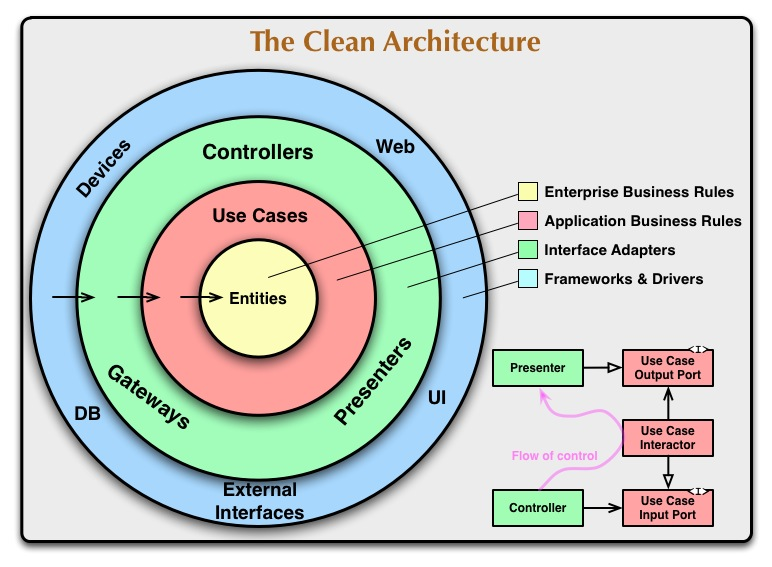
\includegraphics[scale=.55]{immagini/cleanarchitecture.png}
    \caption{Clean Architecture Principle}
    \label{fig:cap}
\end{figure}
Applicare questo principio a Flutter non è proprio come presentato nell'immagine presente sul libro, in quanto non sono propriamente presenti Controller o Gateway, ma l'essenza dell'architettura "pulita" resta lo stesso in qualsiasi framework e quello che faremo è applicarlo a Flutter. Per farlo è stato creato un flusso che i dati dividendo l'applicazioni in tre parti fondamentali, il livello di presentazione, il livello di dominio e il livello dei dati (Figura \ref{fig:architecture})
\begin{figure}
    \centering
    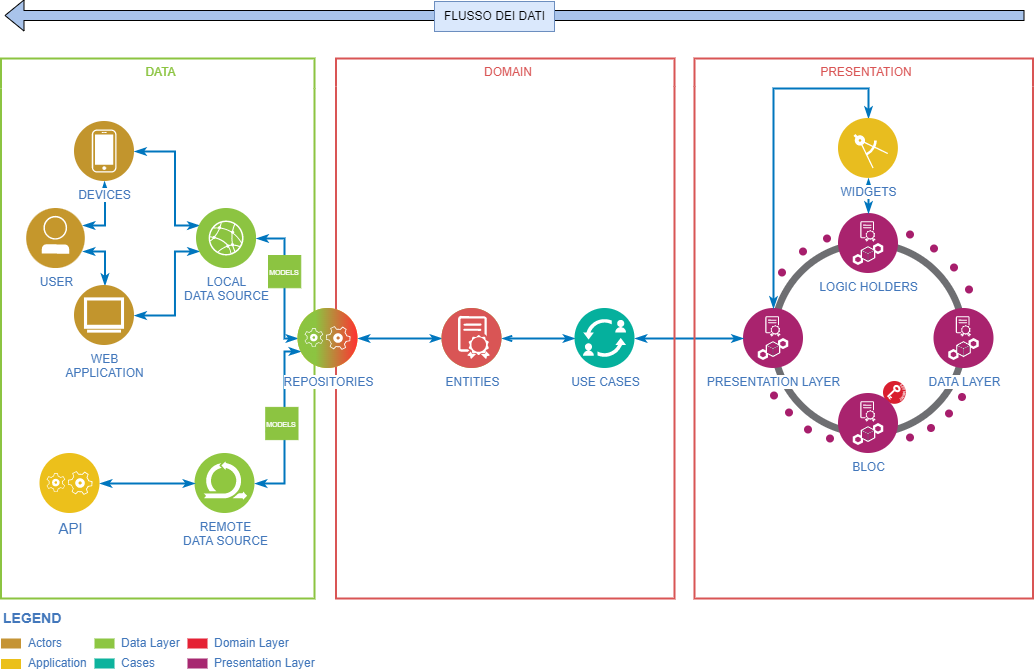
\includegraphics[scale=.42]{immagini/architecture.png}
    \caption{I livelli dell'architettura proposta}
    \label{fig:architecture}
\end{figure}
\subsection{Presentation Layer}
La struttura proposta è anche rispecchiata nei namespace creati all'interno del progetto, nel livello di presentazione possiamo trovare i Widgets, ovvero i componenti principali di flutter per l'interfaccia grafica e Bloc, lo state management scelto per lo sviluppo dell'applicazione.
Il livello di presentazione non farà molto da solo come è solito fare all'interno dei progetti veloci di Flutter, ma effettueranno al massimo qualche controllo sugli input. Tutto il resto verrà delegato al secondo livello ovvero il Domain Layer attraverso gli eventi generati da Bloc (Code Listing \ref{conversation_bloc}).
\begin{lstlisting}[language=dart,caption=Presentation Layer: conversation\_bloc.dart,label=conversation_bloc]
class ConversationBloc extends Bloc<ConversationEvent, ConversationState> {
  final GetConcreteConversation getConcreteConversation;
  final GetRandomConversation getRandomConversation;
  final InputConverter inputConverter;
  ConversationBloc({required GetConcreteConversation concrete,
      required GetRandomConversation random,
      required this.inputConverter})
      : getConcreteConversation = concrete,
        getRandomConversation = random,
        super(Empty()) {
    on<GetConversationForConcreteStringEvent>(
        (event, emit) async => _onConcreteStringEvent(event, emit));
    on<GetConversationForRandomStringEvent>(
        (event, emit) async => _onRandomStringEvent(event, emit));
  }
}
\end{lstlisting}


\subsection{Domain Layer}
Bloc delegherà il lavoro al livello di dominio, il livello di dominio non dovrà essere suscettibile al cambio del livello dei dati, da dove essi provengono, ma sarà completamente indipendente da esso, conterrà solamente la logica di business che verrà eseguita all'interno dei casi d'uso e i business object, ovvero le entità. Gli use cases non sono altro che classi che conterranno tutta la logica di business relativa al particolare caso d'uso.

Dalla figura \ref{fig:architecture} possiamo notare come il domain layer contiene sul bordo le repositories che saranno replicate sia nel domain layer che nel data layer e per continuare a mantenere il grado di indipendenza quello che faremo è utilizzare quello che viene chiamato Dependency Inversion. 

La Dependency Inversion (Code Listing \ref{injection_container}) verrà implementata creando delle classi astratte che definiranno un "contratto" su cosa le repository dovranno fare. Questo, nell'ottica del modello di sviluppo Test-Driven Development ci permette di "mockarle" facilmente senza doversi curare della vera implementazione.

Queste classi verranno poi registrate dal \texttt{ServiceLocator} che si occuperà di effettuare la dependency injection nei vari componenti.

\texttt{import 'package:get\_it/get\_it.dart'} fornisce la classe \texttt{GetIt} che permette di registrare Factory e Singleton con i metodi \texttt{registerFactory}, \texttt{registerSingleton} oppure \texttt{registerLazySingleton} e si può recuperare l'istanza istanziata con il metodo \texttt{.get()} oppure direttamente con la chiamata a funzione dell'istanza, avendo internamente implementato la funzione \texttt{call()}.
\newpage
\begin{lstlisting}[language=dart,caption=injection\_container.dart,label=injection_container]
final sl = GetIt.instance;
Future<void> init() async {
  // Features - Conversation
  //Bloc
  sl.registerFactory(() =>
      ConversationBloc(concrete: sl(), random: sl(), inputConverter: sl()));
  // Use cases
  sl.registerLazySingleton(() => GetConcreteConversation(sl()));
  sl.registerLazySingleton(() => GetRandomConversation(sl()));
  // Repository
  sl.registerLazySingleton<ConversationRepository>(() =>
      ConversationRepositoryImpl(localDataSource: sl(), remoteDataSource: sl(), networkInfo: sl()));
  //Data sources
  sl.registerLazySingleton<ConversationRemoteDataSource>(
      () => ConversationRemoteDataSourceImpl(client: sl()));
  sl.registerLazySingleton<ConversationLocalDataSource>(
      () => ConversationLocalDataSourceImpl(sharePreferences: sl()));
}
\end{lstlisting}

\begin{lstlisting}[language=dart,caption=Data Layer: conversation\_repository\_impl.dart,label=conversation_repository_impl]
import 'package:dartz/dartz.dart';

import '../../../../core/error/failure.dart';
import '../../domain/entities/conversation.dart';
import '../../domain/repositories/conversation_repository.dart';

class ConversationImpl implements ConversationRepository {
  @override
  Future<Either<Failure, Conversation>> getConcreteConversation(int number) {
    // TODO: implement getConcreteConversation
    return null;
  }

  @override
  Future<Either<Failure, Conversation>> getRandomConversation() {
    // TODO: implement getRandomConversation
    return null;
  }
}
\end{lstlisting}
\subsection{Data Layer}
Il livello dei dati definirà come i dati vengono ottenuti e gestiti, la repository nel livello dei dati implementerà il contratto definito in precedenza (Code Listing \ref{code:conversation_repository}) e quindi si passerà dalla classe astratta alla vera e propria implementazione (Code Listing \ref{conversation_repository_impl}) conformandosi al contratto.

In questo modo il livello di dominio non dovrà preoccuparsi su cosa succede dietro le quinte, ma saprà solamente che tipo di dati riceverà che nel nostro caso sarà il testo del blocco di codice ottenuto in modo diretto o randomico in base ai casi d'uso che più in la sono definiti. 

\begin{lstlisting}[language=dart,caption=Domain Layer:conversation\_repository.dart,label=code:conversation_repository]
import 'package:dartz/dartz.dart';

import '../../../../core/error/failures.dart';
import '../entities/conversation.dart';

abstract class ConversationRepository {
  Future<Either<Failure, Conversation>> getConcreteConversation(int number);
  Future<Either<Failure, Conversation>> getRandomConversation();
}
\end{lstlisting}

Nel nostro caso nel livello dei dati c'è sia un Remote Data Source che otterrà i dati dalle API del nostro modello, sia dal Local Data Sources che otterrà i dati in input da parte dell'utente mediante il dispositivo utilizzato, che sia esso un'applicazione Web o Desktop o Mobile. Repository sarà il cervello del Data Layer in quanto deciderà da quale data source e quando prendere i dati. Dalla figura \ref{fig:architecture} possiamo notare come la repository crea l'entità, che nel nostro caso è la risposta dell'API con il blocco di codice in formato testo. I data sources hanno invece in output i models che si occuperanno di gestire oggetti di tipo Json.(Code Listing \ref{code:conversationRemoteDataSourceImpl})

La logica di conversione da json a entità non verrà messa nell'entità ma nei models proprio per garantire il livello di indipendenza dal livello dei dati (Code Listing  \ref{code:model}). Se per esempio il data source desse in output anziché degli oggetti json, un markdown xml, dovremmo poter sostituire il livello dei dati senza preoccuparci di modificare le entità e quindi il livello di dominio.
\newpage
\begin{lstlisting}[language=dart,caption=Data Layer:conversation\_model.dart,label=code:model] 
import '../../domain/entities/conversation.dart';

class ConversationModel extends Conversation {
  const ConversationModel({required text, required number})
      : super(text: text, number: number);
  factory ConversationModel.fromJson(Map<String, dynamic> json) {
    return ConversationModel(text: json['text'], number: json['number']);
  }

  Map<String, dynamic> toJson() {
    return {'text': text, 'number': number};
  }
}
\end{lstlisting}
\begin{lstlisting}[language=dart,caption=Data Layer: comversation\_remote\_data\_source\_impl.dart,label=code:conversationRemoteDataSourceImpl] 
class ConversationRemoteDataSourceImpl implements ConversationRemoteDataSource {
  final http.Client client;
  final url = 'http://localhost:5001/';
  final headers = {'Content-Type': 'application/json'};

  ConversationRemoteDataSourceImpl({required this.client});

  Future<ConversationModel> _getConversationFromUrl(String url) async {
    final response = await client.get(Uri.parse(url), headers: headers);
    if (response.statusCode == 200) {
      return ConversationModel.fromJson(json.decode(response.body));
    } else {
      throw ServerException();
    }
  }

  @override
  Future<ConversationModel> getConcreteConversation(String comment) =>
      _getConversationFromUrl('http://localhost:5001/query=?$comment');

  @override
  Future<ConversationModel> getRandomConversation() =>
      _getConversationFromUrl('http://localhost:5001/random');
}
\end{lstlisting}
\newpage
\subsection{Frontend}
Lato frontend, per ottenere un MVP (Minimum Viable Product) è stata costruita una semplice interfaccia grafica che permetterà, tramite l'utilizzo di due comandi, \texttt{Cerca Funzione} e \texttt{Funzione Casuale} di ottenere rispettivamente, una funzione ricercata in base al testo inserito dall'utente nell'input-box, richiamando il caso d'uso \texttt{getConcreteConversation} ed una funzione casuale ricavata in modo randomico dal dataset, questa racchiude per l'appunto il secondo caso d'uso \texttt{getRandomeConversation}.

In entrambi i casi verrà presentato in output un contenitore base (con scrolling nel caso in cui la funzione sia lunga) con all'interno il codice della funzione ed un ulteriore tasto per copiarne il contenuto ed eventualmente permettere allo sviluppatore di utilizzarlo.

\begin{figure}[h]%
    \centering
    {{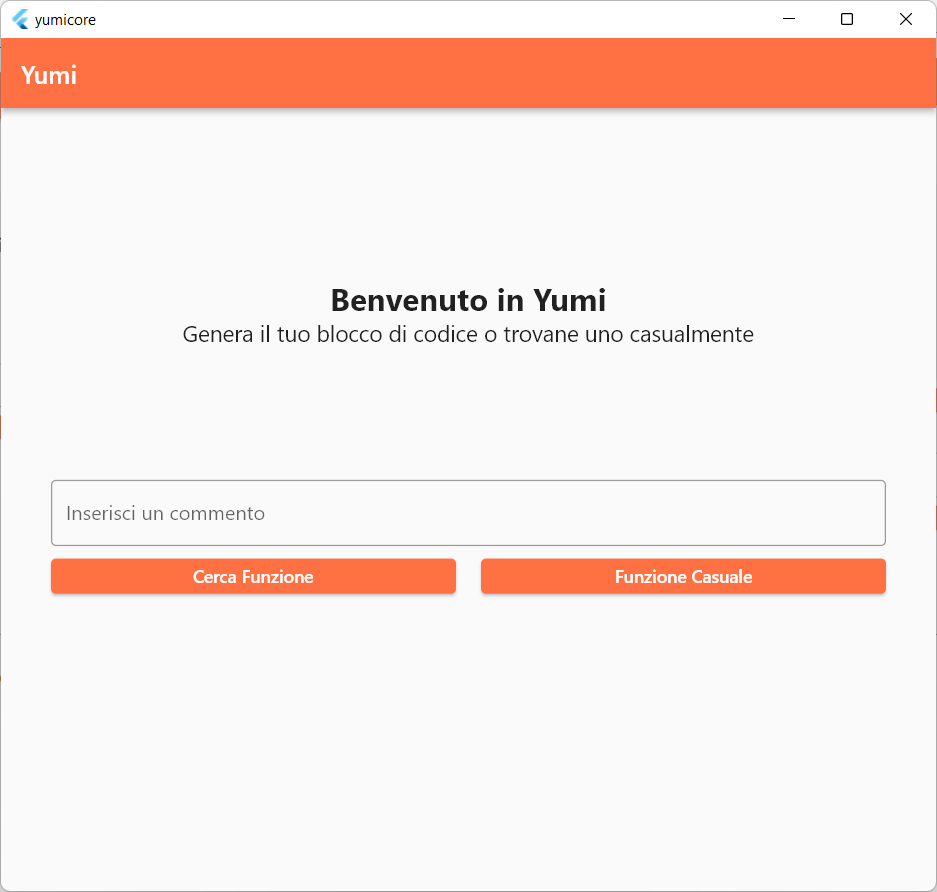
\includegraphics[width=7cm]{immagini/yumi_interface.png} }}%
    \qquad
    {{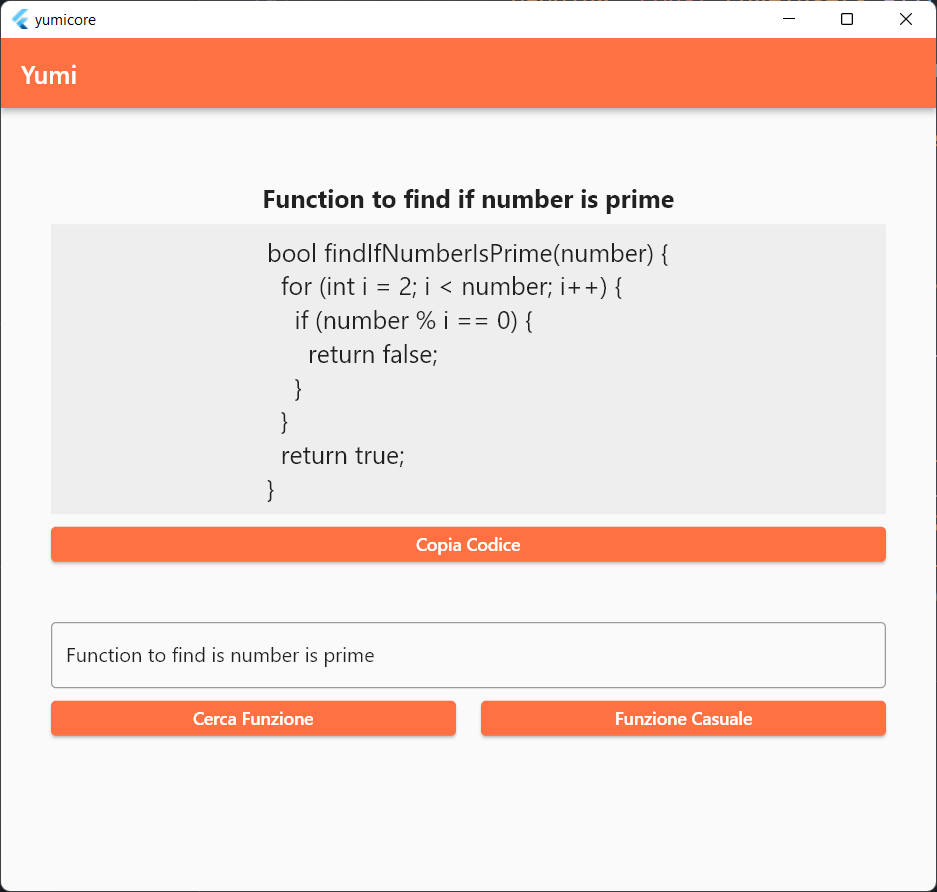
\includegraphics[width=7cm]{immagini/yumi_query.png} }}%
    \caption{Schermata principale di Yumi (sinistra) e codice generato dopo la richiesta (destra)}%
    \label{fig:example}%
\end{figure}

\subsection{Backend}
Lato backend invece, è stato creato un server che tramite Python espone delle API contenenti due endpoint \texttt{random} e \texttt{concrete}. La prima ci permetterà di accedere ad un risultato casuale legato al caso d'uso \texttt{getRandomConversation}, mentre l'ultima restituirà il risultato della query in input ovvero del caso d'uso sopra descritto \texttt{getConcreteConversation}.

Per fare ciò utilizzeremo un server tramite Api RESTFul Flask che risponderà agli URL locali:
\begin{description}
    \item \texttt{GET:} \texttt{http://localhost:5001/random} 
    \item \texttt{GET:} \texttt{http://localhost:5001/query?comment=testoquery} 
\end{description}

\begin{python}
class ConcreteConversation(Resource):
    @use_kwargs({'comment': fields.Str(required=True)},location="query")
    def get(self, comment):
        return {
            "comment": "{}!".format(comment),
            "code": "{}".format(getConcreteConversation(comment))
        }

class RandomConversation(Resource):
    def get(self):
        return getRandomConversation()

# Error handler for Flask-RESTful
@parser.error_handler
def handle_request_parsing_error(err, req, schema, *, error_status_code, error_headers):
    """webargs error handler that uses Flask-RESTful's abort function to return
    a JSON error response to the client.
    """
    abort(error_status_code, errors=err.messages)


if __name__ == "__main__":
    api.add_resource(ConcreteConversation, "/query")
    api.add_resource(RandomConversation, "/random")
    app.run(port=5001, debug=True)
\end{python}
\begin{lstlisting}[frame=none,caption={Un'estratto del codice per l'avvio del server backend in locale},captionpos=b,label=pythonbackendstart]
\end{lstlisting}

Il backend, testato in locale, interagisce con il modello e dal dataset va estrarre in risposta, in formato \texttt{json} commento e codice della funzione trovata.

\begin{lstlisting}[language=json,firstnumber=1]
{
  "comment": "Find if number is prime",
  "code": "  bool findIfNumberIsPrime(int number) {[...]}"
}
\end{lstlisting}
\newpage
\section{Estendibilità e Sviluppi Futuri}
L'utilizzo di quanto visto nel capitolo \ref{section:architecture} e le tecniche di clean architecture descritte nel paragrafo \ref{paragraph:cleanArchitecture} e successivi, danno modo non solo al nostro tool di essere esteso in modo veloce e controllato ma anche di essere riutilizzato per altri scopi. 

L'interfaccia grafica è completamente separata dalla logica di business, i parametri all'interfaccia arrivano tramite lo state manager adottato, nel nostro caso Bloc, ma anch'esso a sua volta è completamente separato dal livello di dominio, quindi è possibile sostituirlo con qualsiasi altro event manager. 

La logica di dominio può essere a sua volta sostituita, andando semplicemente a modificare l'implementazione della repository. Per esempio per cambiare l'API alla quale Yumi fa le richiesta per l'output è immediato, si crea una nuova implementazione della \texttt{ConversationRepository} e la si inietta tramite Dependency Injection all'interno del Service Locator, in poche righe di codice Yumi può diventare un generatore di ricette, oppure un vero e proprio chatbot! E così via anche per il livello dei dati e i modelli, possiamo elaborare XML piuttosto che file JSON in qualche minuto.

\begin{quotation}\small\selectlanguage{english}
\textit{"Non ci vuole poi questa gran conoscenza o abilità per far funzionare un programma. Far funzionare qualcosa, almeno una volta, non è poi così difficile. Far le cose per bene è proprio tutta un'altra cosa. Scrivere un buon software è difficile. Quando il software è fatto bene, la sua creazione e manutenzione richiede solo una frazione delle risorse umane. Ogni modifica è semplice e rapida"}\cite{10.5555/3175742}
\end{quotation}

Non solo, è anche possibile esporre le API direttamente dalla repository piuttosto che interagire con un'interfaccia desktop è possibile far si che Yumi diventi una Web App in pochissime righe di codice. 

Gli sviluppatori spesso credono che il time-to-market sia più importante di una buona architettura, la corsa al rilascio del software è molto presente all'interno dell'informatica ma è anche molto dannosa. Il \textit{"possiamo sempre sistemarlo dopo"} fa tendere la produttività a zero, è importante per questo motivo cercare di uscire sin da subito con idee di struttura del codice ben manutenibile e estensibile e Yumi, anche se è un progetto piccolo sviluppato in singolo, ne è un esempio.